

%*********************************************************************************************************
\section{Introduction}
%*********************************************************************************************************
Along with the emergence of Web 2.0 and services based computing,  the Web has become a software as services development platform for applications. Lambda users have thereby access to different services some exported by their favorite social networks, music and leisure providers.  As in other platforms, the applications' integration problem emerges again  and calls for simple coordination solutions that can give users' a global view of their Web services within a whole, unique and, dynamic space. For example, having an integrated view of the mood of a user according to the status of her favorite social networks. The integration of data services  can be done today by coordinating services accessible on the  network. For example, synchronizing music lists listened in LastFM  with a user account in Twitter and Facebook ({\em status: "Desert Rose - Sting"}) and observe and use this information to determine the degree of music preference convergence of a community of users. Yet, such services produce and update some of these data dynamically (e.g. the status in messenger when the user listens music) and integrated views must be continuously and automatically updated according to specific  requirements: data freshness, periodic and atomic update of data shared among several services despite eventual exceptions.

Current standards in services' coordination implement functional, non-functional properties (NFP) and communication aspects by combining different languages and protocols. WSDL and SOAP among others are languages used respectively for describing services' interfaces and message exchange protocols for calling methods exported by such services. For adding a transactional behaviour to a services' coordination it is necessary to implement WS-Coordination, WS-Transaction, WS-BussinessActivity and WS-AtomicTransaction. The selection of the adequate protocols for adding a specific NFP to a services' coordination (e.g., security, transactional behaviour and adaptability) is responsibility of a programmer. As a consequence, the development of an application based on a services' coordination is a complex and a time-consuming process. This is opposed to the philosophy of services that aims at facilitating the integration of distributed applications. Therefore, in contrast to these approaches, our work is inspired in the philosophy of \textit{separation of concerns} adopted in the construction of middleware for specifying NFP's to a services' coordination in orthogonal way.
%(ii) generating mechanisms for ensuring these properties at services' coordination execution time.

This paper presents a methodology   for ...  to ensure NFP's policies specified by the coordination designer. For example, update the status of all user Facebook, Twitter and Yahoo accounts or maintain the current status if one of them is not accessible.  Thanks to policies associated to a services based application running in a Web dynamic environment, it is possible to associate a personalized behaviour: atomic integration of information retrieved from different social network services, automatic generation of an integrated view of the operations executed in different social networks.

The remainder of the paper is organized as follows. 
%Section \ref{sec:policycoord} introduces our approach for defining policies and associating them to service coordination for adding and ensuring NFP's at execution time. Section \ref{sec:reaction} describes observation and reaction strategies used for monitoring the execution of the coordination and reacting on it according to the policies associated to the coordination. Section \ref{sec:musicmood} describes implementation issues and a validation experience integrating well-known social networks services namely FaceBook, Twitter and, LastFM. 
%The section insists on the synchronization of the messages expressed automatically or explicitly by social network users and then shows how the services are coordinated observed and then synchronized thanks to policies. 
Section \ref{sec:related} analyses related work concerning policy/contract based programming and, service coordination platforms. Section \ref{sec:conclusions} concludes the paper and discusses future work.

%*********************************************************************************************************
\section{Framework overview }\label{sec:approach}
%*********************************************************************************************************
Figure \ref{fig:framework} shows the general overview to the framework we propose for specifying and designing reliable service based applications. The objective   is to model and associate non functional properties to  service based applications that represent both systems' cross-cutting aspects (e.g., exception handling expressing what to do when a service is not available) and use constraints stemming from the services used for implementing them (e.g., the fact that a service requires imposes an authentication protocol for executing a method)  Thus, the framework proposes a meta-modelling approach that  (i) extends the  CIM and PIM ??? layers of the SODM methodology \ref{decastro-etal10} that  provides concepts for modeling services' compositions with the notion of {\sf\small Policy} for representing nonfunctional properties and, (ii) defines  transformation rules for generating concrete reliable service compositions implementations. Service compositions are implemented in a intermediate composition language named PEWS \ref{pews} that provides constructs for expressing the composition and the policies. PEWS expressions are then transformed into Java programs using the PEWS metamodel and transformation rules into Java that we have defined.  


\begin{figure}[htpb]
\begin{center}
%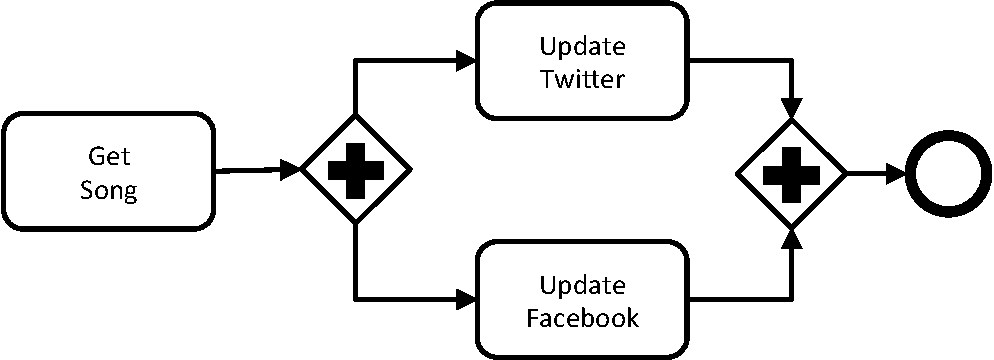
\includegraphics[width=100.0mm]{figs/SC}
\end{center}
		\caption{General overview of the framework}
   \label{fig:framework}

\end{figure}


%*********************************************************************************************************
%\section{Running example}\label{sec:usecase}
%*********************************************************************************************************


Consider for instance the following scenario. An imaginary music provider...

A programmer wants to develop the application Status Broadcaster that estimates the "mood" of people  based on the music they are listening during some periods of time and sends the song title and the mood to Twitter and Facebook. For example, if we consider that people listening to pop-music are "happy" and most songs listened by a person are pop-music, then the application estimates that the person is "happy". Social network users will have their status synchronized in  Twitter and Facebook  with the title of the music they are listening in LastFM (http://www.lastfm.fr/) and the associated mood.
For developing this application the programmer has to coordinate the calls to the methods offered by the following services:
\begin{itemize}
\item Music Services like  LastFM export methods for obtaining information  about the music a given user is listening:
\begin{itemize} \item {\sf\small get-Last-Song ( userid ): String} ; \end{itemize}
\item Facebook and Twitter services export methods for getting and updating the status of a given user: 
\begin{itemize} \item{\sf\small get-Status ( usedid ): String ; \item update-Status ( userid, new-status ): String}; \end{itemize}
\item Mood Service exports a method for retrieving the mood of a  user: 
\begin{itemize} \item{\sf\small get-Mood ( userid ): String} ;\end{itemize}
It is a complex process that uses a log of the music listened by the user in LastFM during some period of time, and then according to the classification of each song it will determine her mood.
\end{itemize}
The corresponding services' coordination is represented by the workflow depicted in Figure \ref{fig:musicmoodwk} using BPMN \footnote{Details on BPMN (Business Process Management Notation) can be found in http://www.bpmn.org/}.
\begin{figure}[htpb]
\begin{center}
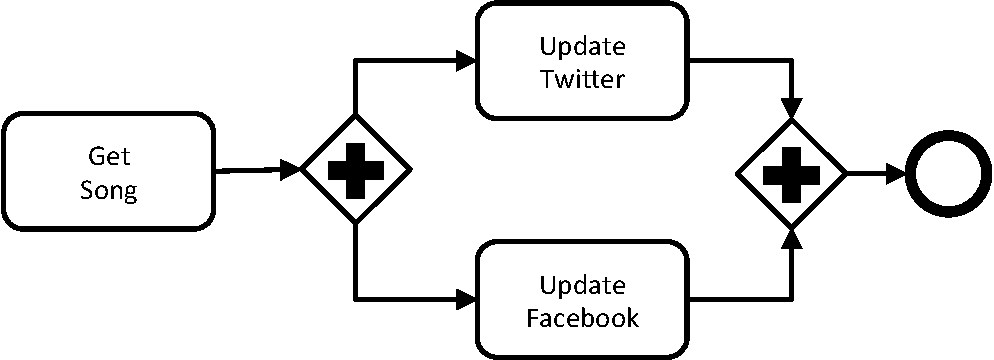
\includegraphics[width=100.0mm]{figs/SC}
\end{center}
		\caption{Status Broadcaster process expressed as a workflow}
   \label{fig:musicmoodwk}

\end{figure}
As shown in the Figure, the process Status Broadcaster starts by contacting the music service LastFM for retrieving the user's  musical status. This information is sent to the mood service in order to calculate the mood of the user. Therefore, the Twitter and Facebook services are called for retrieving the status of the user which is compared with other analysis data in order to determine the mood.  This process is not explicitly expressed in the Figure, it is implemented by the complex activity Compute Mood  (see the C. Activity representation in the Figure  \ref{fig:musicmoodwk}).  Finally, Twitter and Facebook services are contacted in parallel for updating the user's status with the corresponding song and mood. 

Now consider that the Facebook and Twitter services require authentication protocols in order to execute methods that will read and update the users' space. When these services are called by activities of a coordination the call must be part of the authentication protocol required by these services.  Some services use the http authentication protocol that consists in providing the login and password of the user within the communication protocol. Once the access granted it is possible to read and write the status content  of the user's wall.   Twitter and Facebook use the open authentication protocol that consists in making participate a confidence tier that provides a token for granting access to a user's account. In the following we focus the notion of policy used for specifying the authentication protocols for  services' coordinations. 

%..--..--..--..--..--..--..--..--..--..--..--..--..--..--..--..--..--..--..--..--..--..--..--..--..--..--..--..--..--..--..--..--..--..--..--..--..--..--
\subsection{E3value model}
%..--..--..--..--..--..--..--..--..--..--..--..--..--..--..--..--..--..--..--..--..--..--..--..--..--..--..--..--..--..--..--..--..--..--..--..--..--..--

\begin{figure}        
\centering  
%\fbox{
%\epsfig{file=soa.png, height=1.5in, width=2.1in}
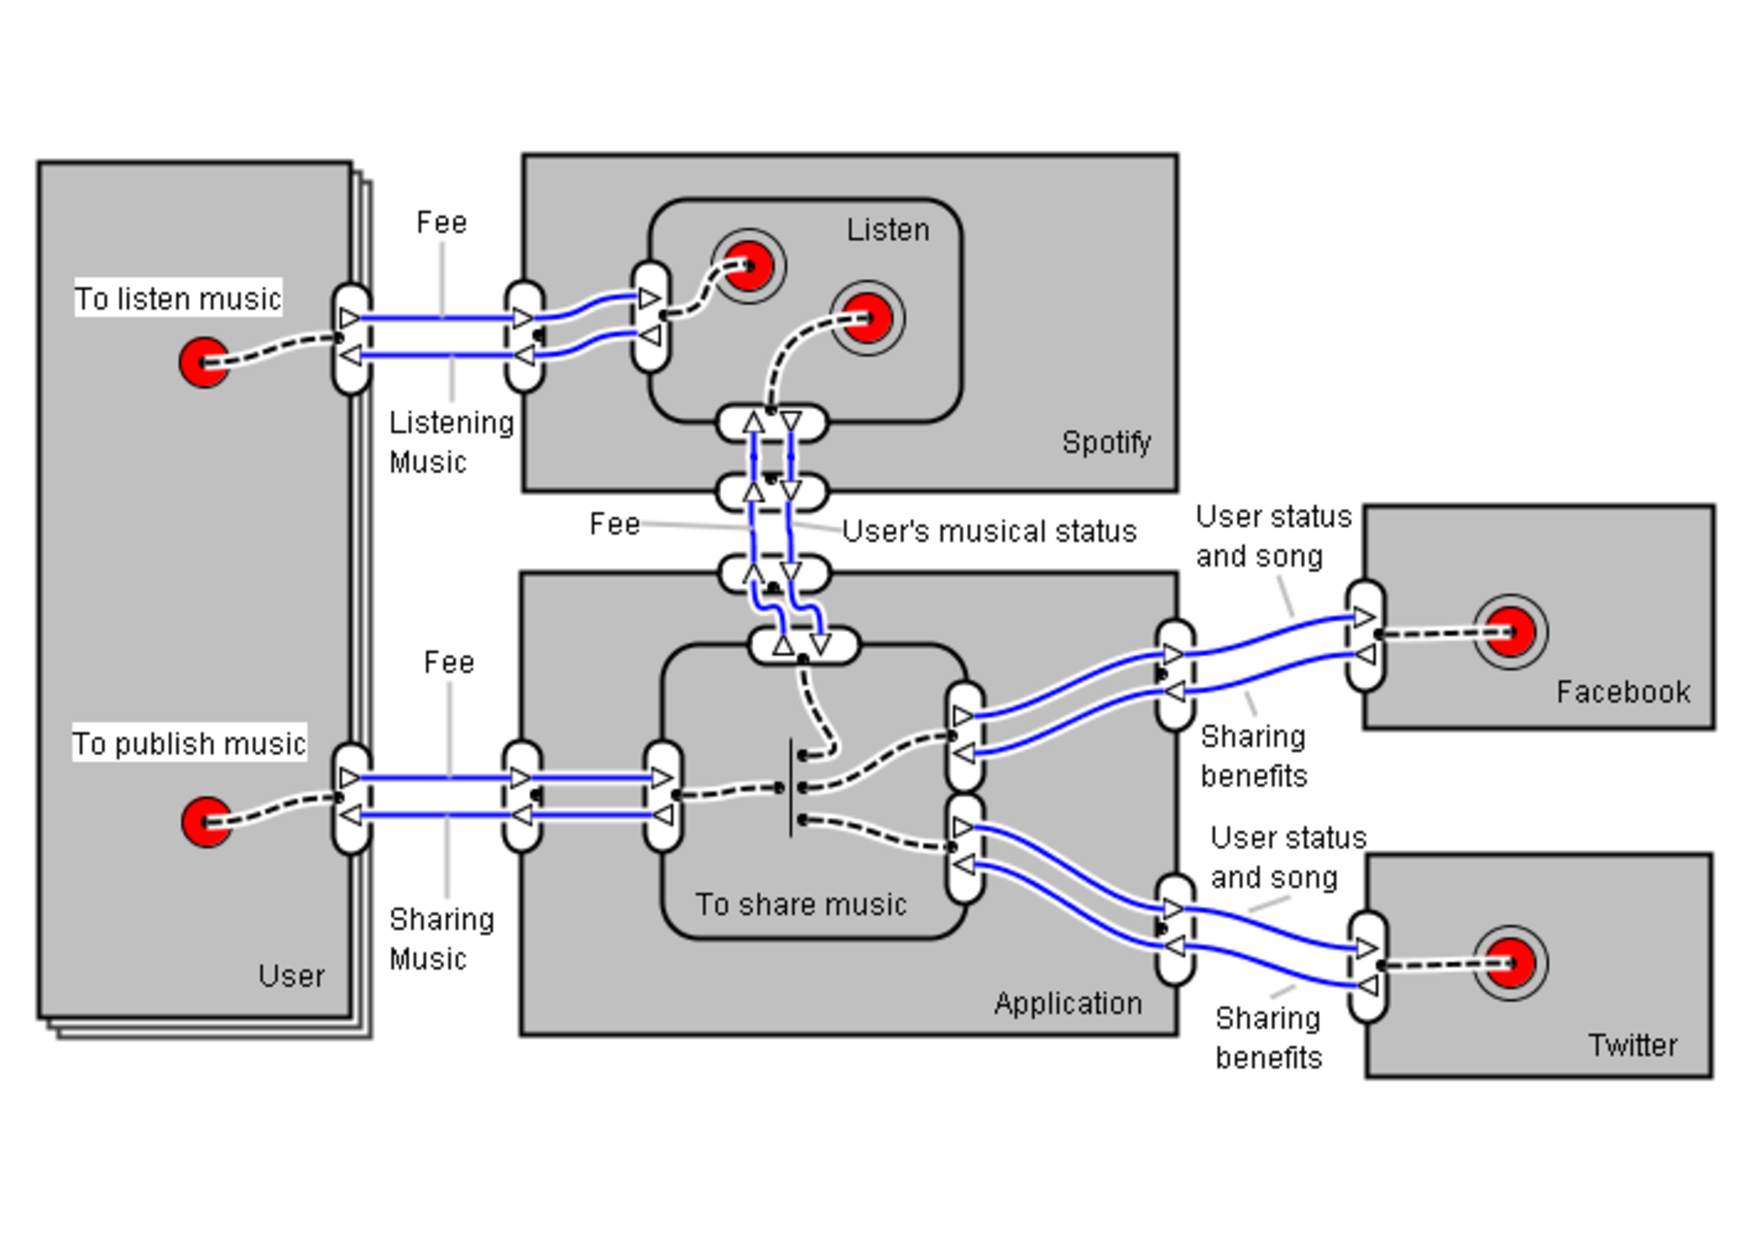
\includegraphics[width=0.60\textwidth]{figs/e3value}
%height=2in, width=2in
%}
\caption{E3value model of the Music-shop scenario.} 
\label{fig:E3valuemodel}
\end{figure}


\begin{figure}        
\centering  
%\fbox{
%\epsfig{file=soa.png, height=1.5in, width=2.1in}
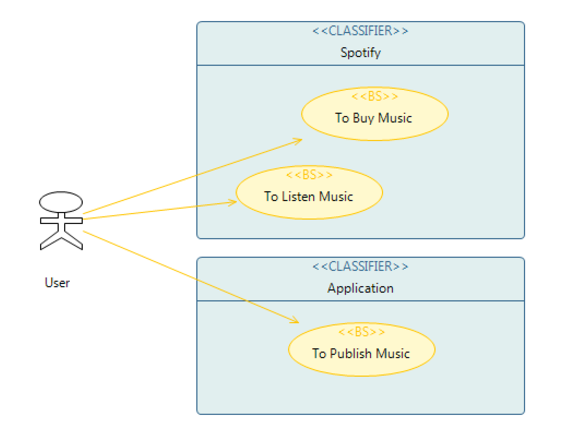
\includegraphics[width=0.60\textwidth]{figs/BS-Model}
%height=2in, width=2in
%}
\caption{Use case diagram of the scenario} 
\label{fig:usecase}
\end{figure}

%..--..--..--..--..--..--..--..--..--..--..--..--..--..--..--..--..--..--..--..--..--..--..--..--..--..--..--..--..--..--..--..--..--..--..--..--..--..--
\subsection{Service composition model}
%..--..--..--..--..--..--..--..--..--..--..--..--..--..--..--..--..--..--..--..--..--..--..--..--..--..--..--..--..--..--..--..--..--..--..--..--..--..--

\begin{figure}        
\centering  
%\fbox{
%\epsfig{file=soa.png, height=1.5in, width=2.1in}
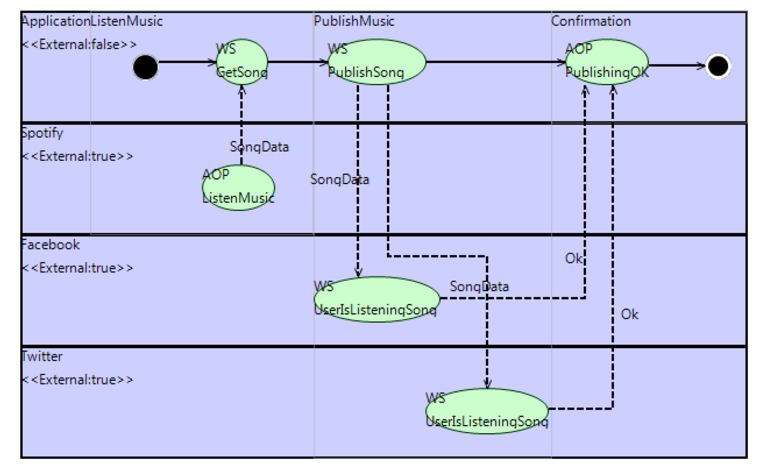
\includegraphics[width=0.80\textwidth]{figs/Composition-Model}
%height=2in, width=2in
%}
\caption{Service composition model} 
\label{fig:servicecompositionmodel}
\end{figure}



%*********************************************************************************************************
\section{Reliable SODM}\label{sec:sodm}
%*********************************************************************************************************
Explanation of the extension of the SODM

%._._._._._._._._._._._._._._._._._._._._._._._._._._._._._._._._._._._._._._._._._._._._._._._._._._._._
\subsection{Stereotyped SODM}
%._._._._._._._._._._._._._._._._._._._._._._._._._._._._._._._._._._._._._._._._._._._._._._._._._._._._

%._._._._._._._._._._._._._._._._._._._._._._._._._._._._._._._._._._._._._._._._._._._._._._._._._._._._
\subsection{Policy}
%._._._._._._._._._._._._._._._._._._._._._._._._._._._._._._._._._._._._._._._._._._._._._._._._._._._._
Figure \ref{fig:policymodel} shows the UML class diagram of our A-Policy model. As shown in the diagram an {\sc A-Policy} is applied to a {\sc Scope} that can be either an {\sc Activity}, an {\sc Operator}, a {\sc Workflow} or a {\sc Policy}. 
It groups a set of ECA rules, each rule having a classic semantics, i.e, {\em when an event of tye E occurs if  condition C is verified then execute the action A}.  Thus, an A-Policy represents a set of re-actions to be possibly executed if one or several triggering events of its rules are notified. 

\begin{figure}[htpb]
	\begin{center}
		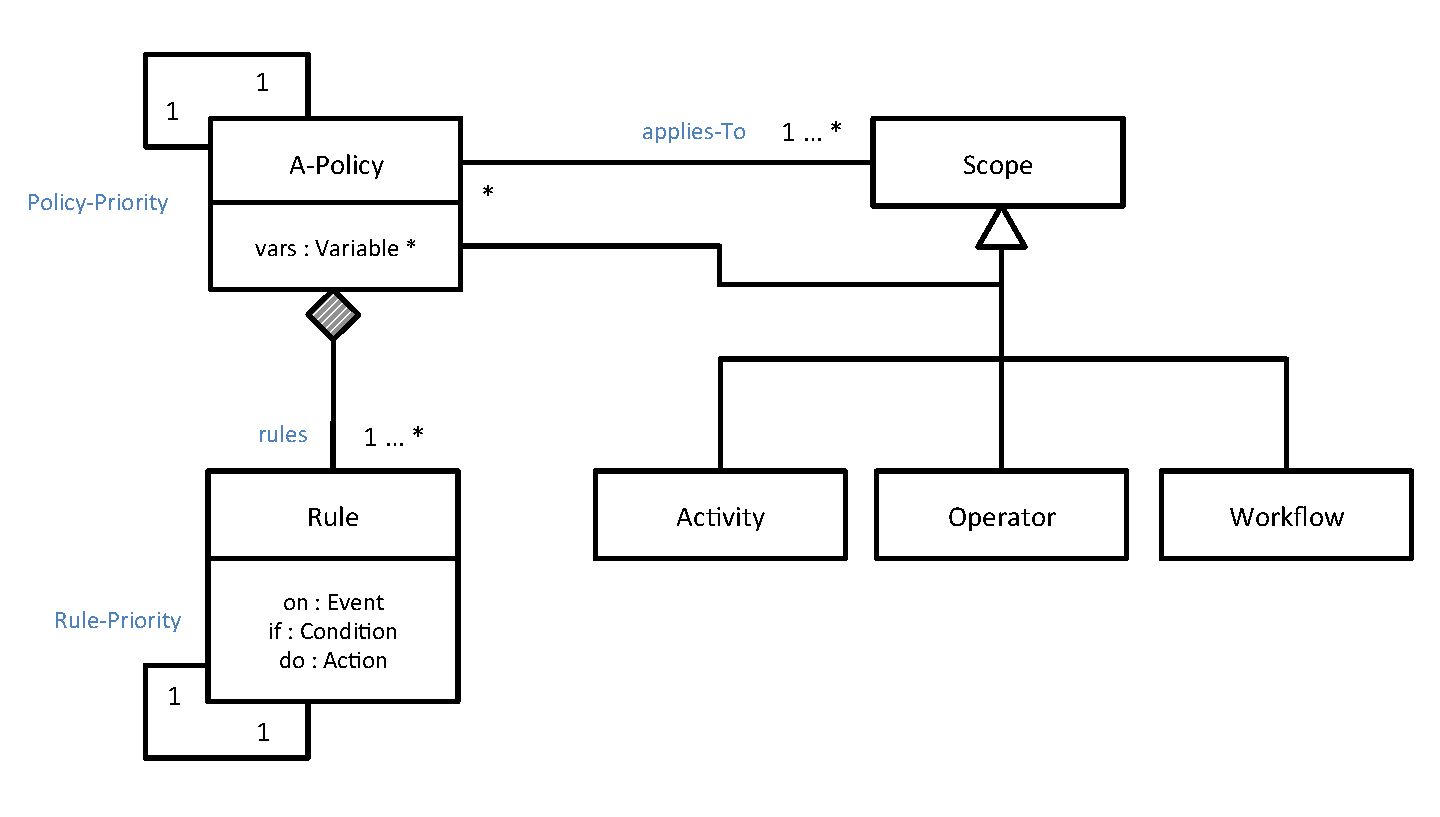
\includegraphics[width=110.0mm]{Figures/AP}
	\end{center}
		\caption{UML class diagram of the A-Policy Model}
   \label{fig:policymodel}
\end{figure}

\begin{itemize}
\item The class {\sc Scope} represents any element of a services' coordination (i.e., activity, operator, workflow).
%a process as an ordered set of execution states  as a set of values of the variables of the execution state of a services' coordination at instant t (or timestamp). The states of a scope are ordered with respect to their timestamps. 

\item The class {\sc A-Policy} represents a recovery strategy implemented by ECA rules of the form {\sc Event} - {\sc Condition} - {\sc Action}. A policy has variables that represent the view of the execution state of its associated scope, that is required for executing the rules. The value of a variable is represented using the type Variable.
\end{itemize}

%*********************************************************************************************************
\section{PEWS metamodel}\label{sec:pewsmetamodel}
%*********************************************************************************************************

Figure \ref{fig:metamodel} presents the PEWS-CT metamodel. Each class refers to
the language terms that can be expressed with it. The structure of the metamodel
has its beginning in the representation of the object \textit{PEWS-CT
Specification}. This class is directly linked to three other classes, they are:
\textit{Namespace, Variable} and \textit{Path Expression}. That classes, in
figure \ref{fig:pews} it are represented in the lines (\textit{1-3, 18-19} and
\textit{32}), respectively.  

A question could be made. How about the operations and services also expressed
in the specification, why they are not directly related to the class
\textit{PEWS-CT Specification}? The answer is because every operation and
service, is directly connected to a namespace. The operations and their
compositions do not exist without the \textit{namespaces}. 



\begin{figure}        
\centering  
%\fbox{
%\epsfig{file=soa.png, height=1.5in, width=2.1in}
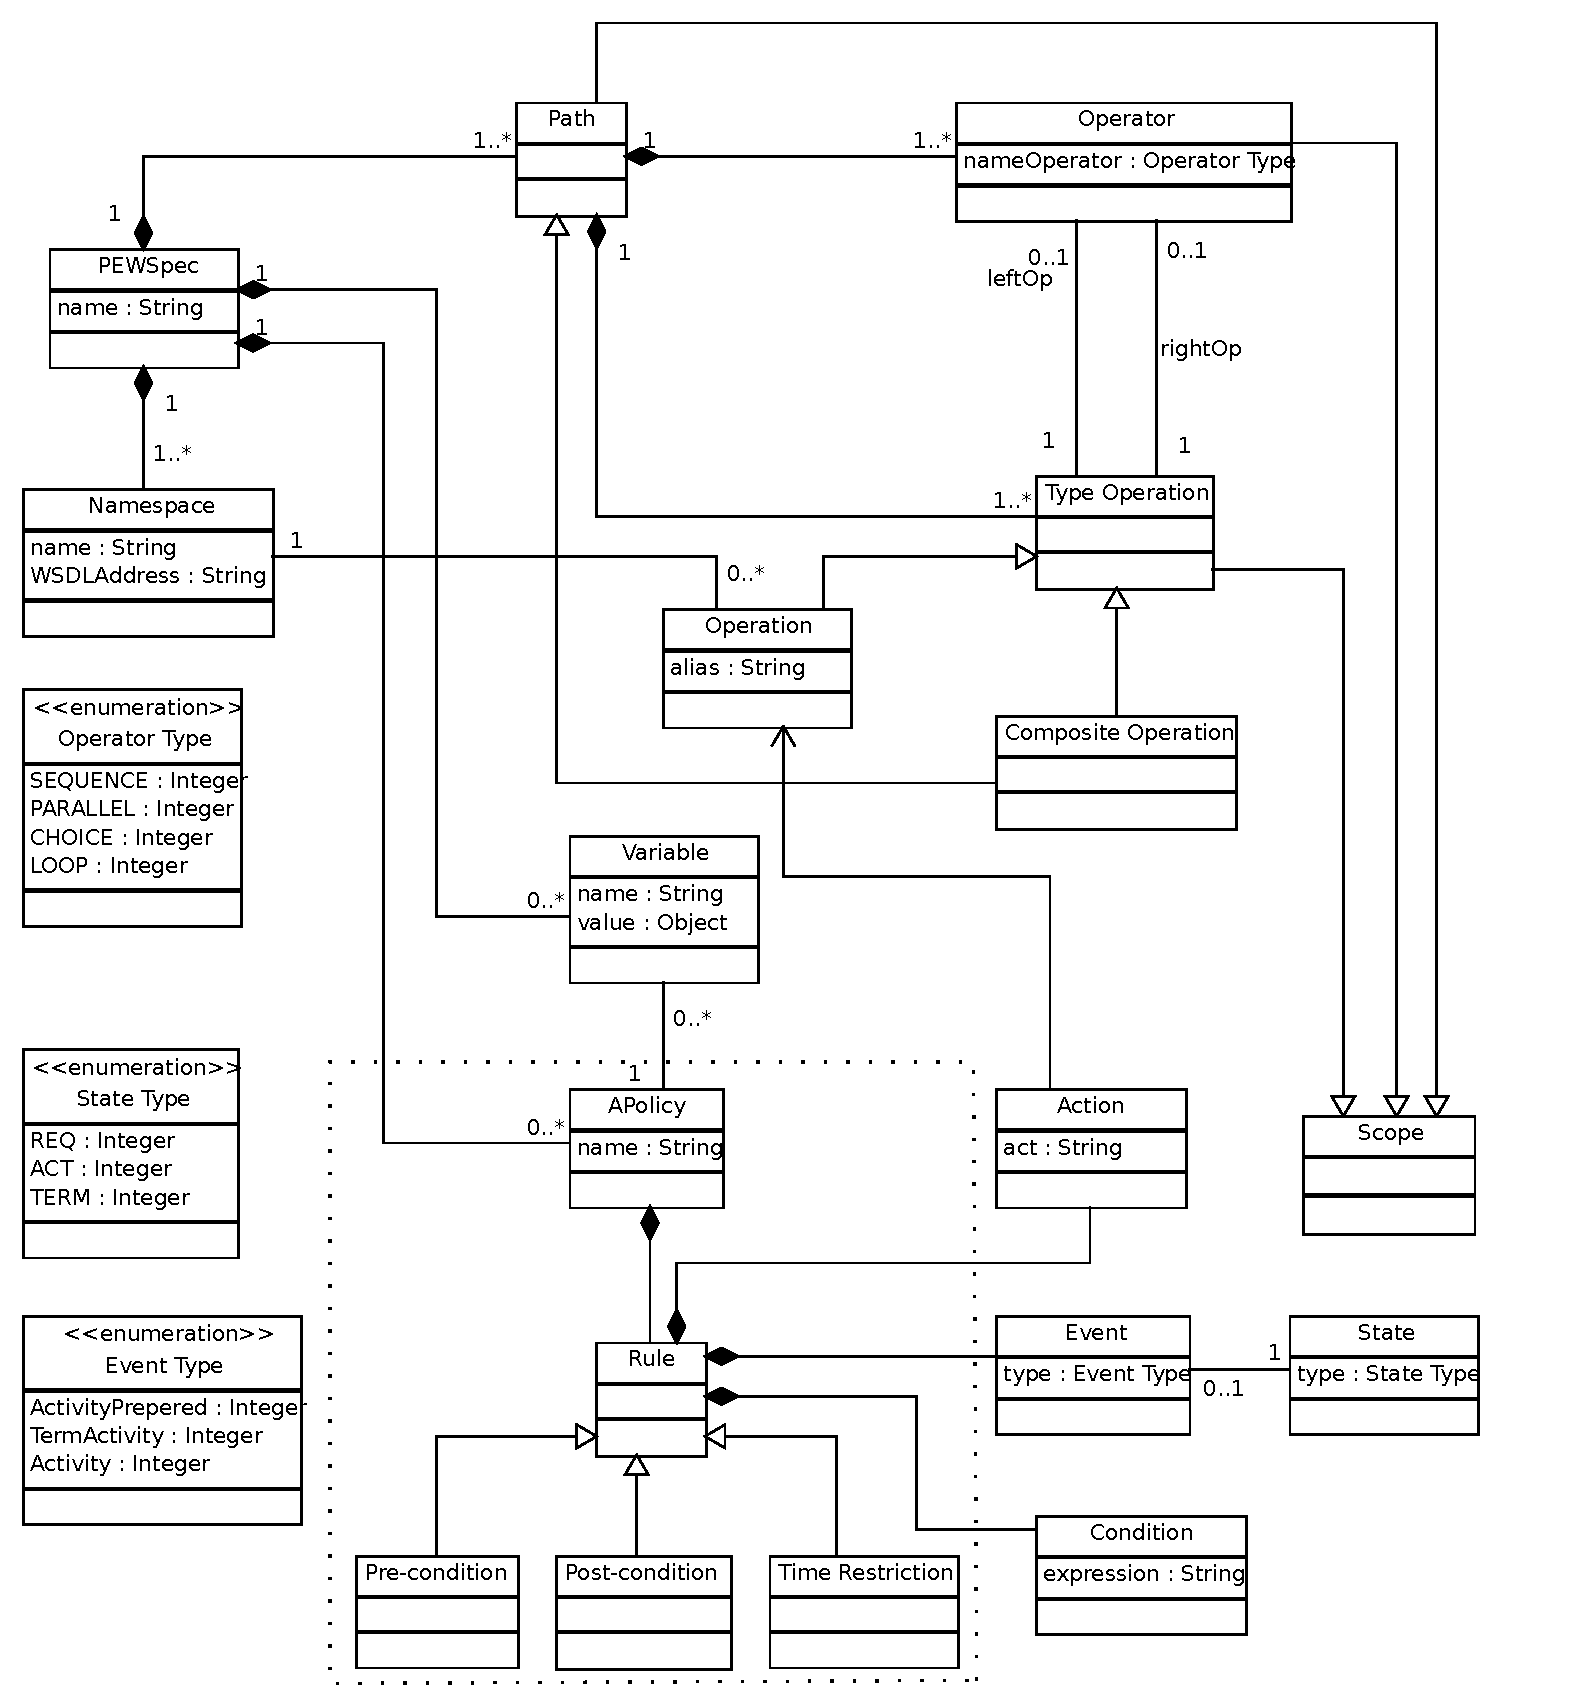
\includegraphics[width=0.99\textwidth]{figs/PEWSMetamodel.png}
%height=2in, width=2in
%}
\caption{PEWS-CT Metamodel.} 
\label{fig:metamodel}
\end{figure}


The \textit{Service} class abstracts both, a single \textit{Operation} and a
composition (\textit{Operation Composition}) represented by the service clause
in PEWS-CT. A \textit{Operation Composition} is a aggregation of one or more
\textit{Operations}. All services have one \textit{Alias} and are composed using
different \textit{Composition Operator}, such as \textit{sequence, parallel,
choice} and so on.  

Each service has zero or more \textit{Contract}s. A contract is a composition of
\textit{Constraint Condition}, that can be as pre-condition, post-condition or
time restriction. A contract condition, if necessary, can performs an
\textit{Action}. An action can be a call to another service; throws an
exception; or stop the process.

The \textit{Constraint Set} is the role constraint in a requires or ensures
clause (figure \ref{fig:pewscontract} ,lines 3-5 and 7), while a \textit{Constraint} is
a single \textit{Expression}, that can be unary or not.
 

%*********************************************************************************************************
\section{Implementation issues}\label{sec:musicmood}
%*********************************************************************************************************
We conducted an implementation of the Status Broadcaster application for synchronizing the status of users in different social networks. We used the Windows Workflow Foundation runtime environment and its underlying notification service that enables us to couple the policies execution. 

The workflow is a simplified version of our example that retrieves the music listened by a user on LastFM and then it atomically updates the status of the user's account in Facebook and Twitter  and it stores the status in a log. This means that if one of the services is not available, the call is compensated. For doing so, the status is updated with the previous one and then the coordination starts again. Figure \ref{fig:musicmoodpolicies}  shows the policies that implement these aspects. They are expressed using our policy language that includes constructs for expressing event types (simple and compound) in the ON part and simple programs in the DO part of the policy rules. Policies are classes of type {\sc a-policy} and they have a scope of type {\sc Activity}, {\sc Workflow} and, {\sc Policy}.

\begin{figure*}
\begin{center}
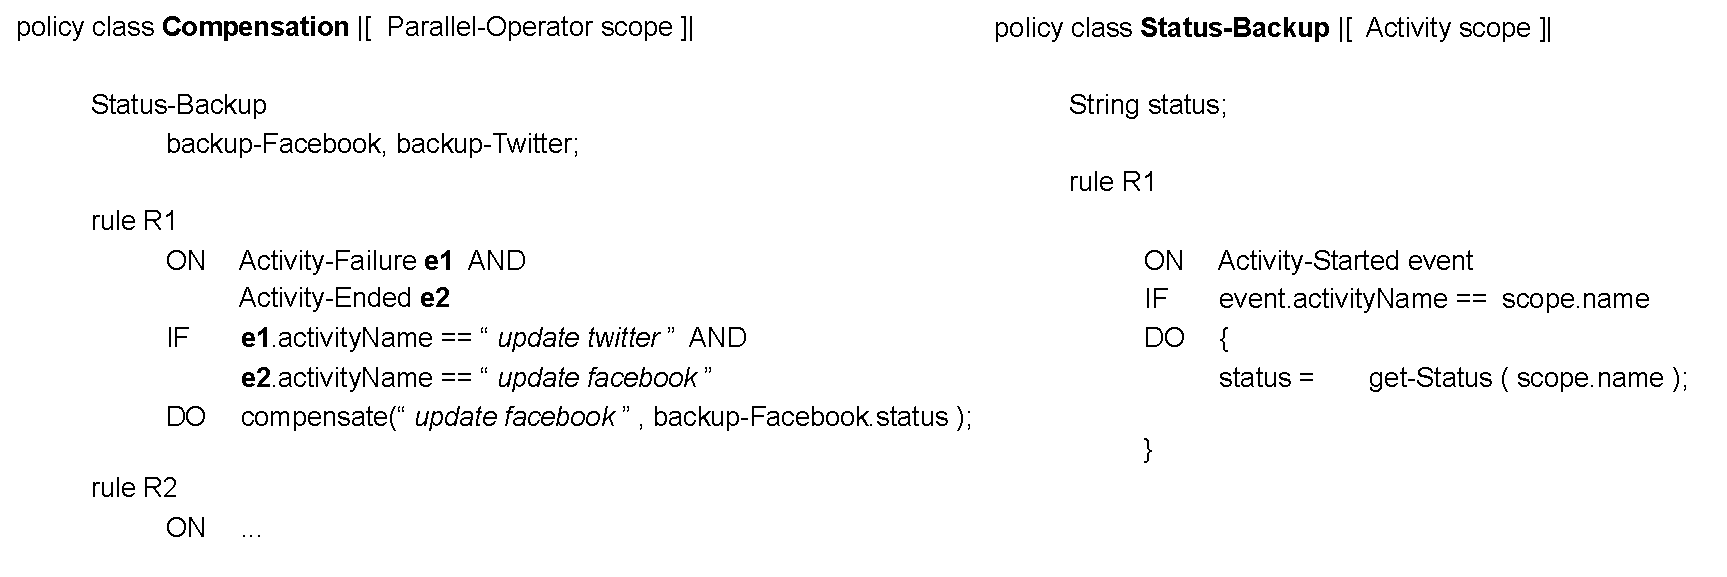
\includegraphics[scale=.50]{figs/Policies}
\end{center}
		\caption{Status broadcaster policies}
   \label{fig:musicmoodpolicies}
\end{figure*}

The policy {\sc\small Compensation} in Figure \ref{fig:musicmoodpolicies} is associated to the parallel operator and handles an exception of any of the activities {\sc\small Update Facebook/Twitter}   compensating it. Therefore it uses the backup status   retrieved by the {\sf\small Status Backup } policy for updating the status in the user wall. The policy {\sc\small Status-Backup} logs the status used for updating the FaceBook and Twitter.

%Given a services' coordination and a set of policies, we generate the code for evaluating every policy as well as the synchronization interface to interact with the services' coordination execution-engine. 
%(see Figure  \ref{fig:9}). 
%A policy-compiler validates whether type declarations and policy expressions are well formed and implements transformation rules for generating classes. The components of a policy-engine import these classes and implement evaluation strategies for executing the policies. The classes implementing the event-types are used for defining the synchronization interface since event detection and event notification are specified on this interface. The classes implementing the actions are used by the policy-engine for synchronizing the execution of services' coordination through the synchronization interface.
%The policy engine consists of a set of components (coordinated by the N-FP Evaluator component) that can be specialized for evaluating policies. The policy evaluation process must be synchronized with a services� coordination. Thus, the policy engine interacts with an coordination engine through a synchronization interface. This interface is a complex component that implements messages based asynchronous communication, where an event type represents a message. 

%._._._._._._._._._._._._._._._._._._._._._._._._._._._._._._._._._._._._._._._._._._._._._._._._._._._._
\subsection{EMF SODM/PEWS}
%._._._._._._._._._._._._._._._._._._._._._._._._._._._._._._._._._._._._._._._._._._._._._._._._._._._._

%._._._._._._._._._._._._._._._._._._._._._._._._._._._._._._._._._._._._._._._._._._._._._._._._._._._._
\subsection{Transformation M-M}
%._._._._._._._._._._._._._._._._._._._._._._._._._._._._._._._._._._._._._._._._._._._._._._._._._._._._

%._._._._._._._._._._._._._._._._._._._._._._._._._._._._._._._._._._._._._._._._._._._._._._._._._._._._
\subsection{Transformation PIM - PCM}
%._._._._._._._._._._._._._._._._._._._._._._._._._._._._._._._._._._._._._._._._._._._._._._._._._._._._


%*********************************************************************************************************
\section{Related works}\label{sec:related}
%*********************************************************************************************************



%*********************************************************************************************************
\section{Conclusions and future work}\label{sec:conclusions}
%*********************************************************************************************************

